% ============================================================
%  PRESENTASI SEMINAR — Artikel MERLIN
%  Journal of Quantitative Spectroscopy & Radiative Transfer
%  330 (2025) 109222
%  A. Favre et al.
%  Dipresentasikan oleh: [Nama Mahasiswa]
% ============================================================
\documentclass[aspectratio=169, 10pt]{beamer}

% ── Tema & Warna ─────────────────────────────────────────────
\usetheme{Madrid}
\usecolortheme{default}
\setbeamercolor{palette primary}{bg=blue!80!black, fg=white}
\setbeamercolor{palette secondary}{bg=blue!60!black, fg=white}
\setbeamercolor{palette tertiary}{bg=blue!40!black, fg=white}
\setbeamercolor{palette quaternary}{bg=blue!20!black, fg=white}
\setbeamercolor{structure}{fg=blue!70!black}
\setbeamercolor{block title}{bg=blue!75!black, fg=white}
\setbeamercolor{block body}{bg=blue!5!white}
\setbeamercolor{block title alerted}{bg=red!75!black, fg=white}
\setbeamercolor{block body alerted}{bg=red!5!white}
\setbeamercolor{block title example}{bg=green!50!black, fg=white}
\setbeamercolor{block body example}{bg=green!5!white}

% ── Font & Bahasa ──────────────────────────────────────────
\usepackage[T1]{fontenc}
\usepackage[utf8]{inputenc}
\usepackage{lmodern}

% ── Paket Sains & Matematika ──────────────────────────────
\usepackage{amsmath, amssymb, physics}
\usepackage{siunitx}
\usepackage{chemformula}
\usepackage{booktabs}
\usepackage{multirow}
\usepackage{array}
\usepackage{xcolor}
\usepackage{tikz}
\usetikzlibrary{arrows.meta, shapes.geometric, positioning, shadows}
\usepackage{pgfplots}
\pgfplotsset{compat=1.18}

% ── Layout ───────────────────────────────────────────────
\usepackage{graphicx}
\usepackage{hyperref}
\usepackage{textcomp}
\setbeamertemplate{navigation symbols}{}
\setbeamertemplate{footline}{%
  \leavevmode%
  \hbox{%
    \begin{beamercolorbox}[wd=.33\paperwidth,ht=2.5ex,dp=1.5ex,center]{palette primary}%
      \usebeamerfont{author in head/foot}\insertshortauthor
    \end{beamercolorbox}%
    \begin{beamercolorbox}[wd=.34\paperwidth,ht=2.5ex,dp=1.5ex,center]{palette secondary}%
      \usebeamerfont{title in head/foot}\insertshorttitle
    \end{beamercolorbox}%
    \begin{beamercolorbox}[wd=.33\paperwidth,ht=2.5ex,dp=1.5ex,right]{palette tertiary}%
      \usebeamerfont{date in head/foot}\insertframenumber/\inserttotalframenumber\hspace{1em}
    \end{beamercolorbox}}%
}

% ── Metadata Presentasi ──────────────────────────────────
\title[MERLIN: LTE Radiative Transfer Code]%
  {\textbf{MERLIN}\\[4pt]
   \textit{An Adaptive LTE Radiative Transfer Model for Any Mixture}\\[2pt]
   \small Validation on Eurofer97 in Argon Atmosphere}

\subtitle{\small\textit{Journal of Quantitative Spectroscopy \& Radiative Transfer}, 330 (2025) 109222}

\author[A. Favre et al.]{%
  \textbf{A. Favre, B. Brioude, A. Bultel}\\[2pt]
  \small CORIA UMR 6614 -- Normandie Univ., CNRS, INSA \& Univ. Rouen\\
  \small \texttt{Journal of Quantitative Spectroscopy \& Radiative Transfer}
}

\date{Dipresentasikan: April 2026}

% ── Makro Berguna ─────────────────────────────────────────
\newcommand{\kB}{k_{\mathrm{B}}}
\newcommand{\nele}{n_e}
\newcommand{\Te}{T}
\newcommand{\epsla}{\epsilon_\lambda}
\newcommand{\alpla}{\alpha_\lambda}
\newcommand{\Wla}{\Delta\lambda}
\newcommand{\highlight}[1]{\textcolor{blue!80!black}{\textbf{#1}}}
\newcommand{\redalert}[1]{\textcolor{red!70!black}{\textbf{#1}}}

% ══════════════════════════════════════════════════════════════
\begin{document}
% ══════════════════════════════════════════════════════════════

% ── Halaman Judul ──────────────────────────────────────────
\begin{frame}[plain]
  \titlepage
\end{frame}

% ── Outline ────────────────────────────────────────────────
\begin{frame}{Outline Presentasi}
  \tableofcontents
\end{frame}

% ──────────────────────────────────────────────────────────
\section{Pendahuluan}
% ──────────────────────────────────────────────────────────

\begin{frame}{Latar Belakang: LIBS \& Tantangannya}
  \begin{columns}[T]
    \begin{column}{0.55\textwidth}
      \begin{block}{Laser-Induced Breakdown Spectroscopy (LIBS)}
        \begin{itemize}
          \item Teknik analisis multi-elemen via emisi plasma laser
          \item Dapat menganalisis padatan, cairan, gas
          \item Dua pendekatan kuantifikasi:
            \begin{enumerate}
              \item \highlight{Calibrated LIBS} — memerlukan sampel referensi
              \item \highlight{Calibration-Free LIBS (CF-LIBS)} — menggunakan model fisika LTE
            \end{enumerate}
        \end{itemize}
      \end{block}
      \vspace{4pt}
      \begin{alertblock}{Masalah Utama}
        Sampel kompleks (paduan tak diketahui, konsentrasi bervariasi) $\Rightarrow$ kalibrasi konvensional tidak memadai
      \end{alertblock}
    \end{column}
    \begin{column}{0.42\textwidth}
      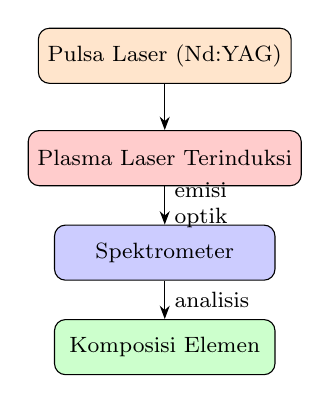
\begin{tikzpicture}[>=Stealth, font=\footnotesize]
        \node[draw, fill=orange!20, rounded corners, minimum width=2.8cm, minimum height=0.7cm]
              (laser) at (0,3.5) {Pulsa Laser (Nd:YAG)};
        \node[draw, fill=red!20, rounded corners, minimum width=2.8cm, minimum height=0.7cm]
              (plasma) at (0,2.2) {Plasma Laser Terinduksi};
        \node[draw, fill=blue!20, rounded corners, minimum width=2.8cm, minimum height=0.7cm]
              (spec) at (0,1.0) {Spektrometer};
        \node[draw, fill=green!20, rounded corners, minimum width=2.8cm, minimum height=0.7cm]
              (comp) at (0,-0.2) {Komposisi Elemen};
        \draw[->] (laser) -- (plasma);
        \draw[->] (plasma) -- node[right, align=left]{emisi\\optik} (spec);
        \draw[->] (spec) -- node[right]{analisis} (comp);
      \end{tikzpicture}
    \end{column}
  \end{columns}
\end{frame}

\begin{frame}{Kontribusi Utama Artikel}
  \begin{block}{Kontribusi Penelitian}
    Artikel ini memperkenalkan kode simulasi plasma spektroskopi
    bernama \textbf{MERLIN} yang digunakan untuk rekonstruksi spektrum
    pada teknik \textit{Calibration-Free Laser-Induced Breakdown
    Spectroscopy (CF-LIBS)}.
  \end{block}

  \begin{itemize}
    \item Pengembangan \textbf{radiative transfer code} berbasis LTE
    \item Generasi adaptif spesies plasma untuk campuran unsur kompleks
    \item Integrasi otomatis dengan \textbf{database spektral online}
    \item Validasi model menggunakan eksperimen LIBS pada
          paduan \textbf{Eurofer97}
  \end{itemize}

  \vspace{6pt}
  \begin{alertblock}{Tujuan}
    Merekonstruksi spektrum plasma LIBS tanpa parameter penyesuaian
    bebas (\textit{no adjustable parameters}).
  \end{alertblock}
\end{frame}

\begin{frame}{Solusi: Kode MERLIN}
  \begin{block}{\textbf{MERLIN} --- \textit{MultiElemental Radiative equiLibrIum emissioN}}
    \begin{itemize}
      \item Kode transfer radiasi berbasis \textbf{Local Thermodynamic Equilibrium (LTE)}
      \item Mampu memodelkan \textbf{campuran elemen apapun} secara adaptif
      \item Kueri otomatis dari \textbf{database spektral online} (NIST, dll.)
      \item Dioptimasi dengan \textbf{paralelisasi} dan \textbf{vektorisasi}
    \end{itemize}
  \end{block}

  \vspace{6pt}
  \begin{columns}[T]
    \begin{column}{0.48\textwidth}
      \begin{exampleblock}{Keunggulan Utama}
        \begin{itemize}
          \item Tanpa variabel penyesuaian (\textit{no adjusted variable})
          \item Spesies poliatom didukung
          \item Komputasi di mesin kapasitas rendah
        \end{itemize}
      \end{exampleblock}
    \end{column}
    \begin{column}{0.48\textwidth}
      \begin{exampleblock}{Target Aplikasi}
        \begin{itemize}
          \item CF-LIBS pada paduan kompleks
          \item Sampel uji: Eurofer97 (baja reduksi aktivasi)
          \item Atmosfer: Argon (\SI{5e4}{Pa})
        \end{itemize}
      \end{exampleblock}
    \end{column}
  \end{columns}
\end{frame}

\begin{frame}{Arsitektur Model MERLIN}
  \begin{center}
    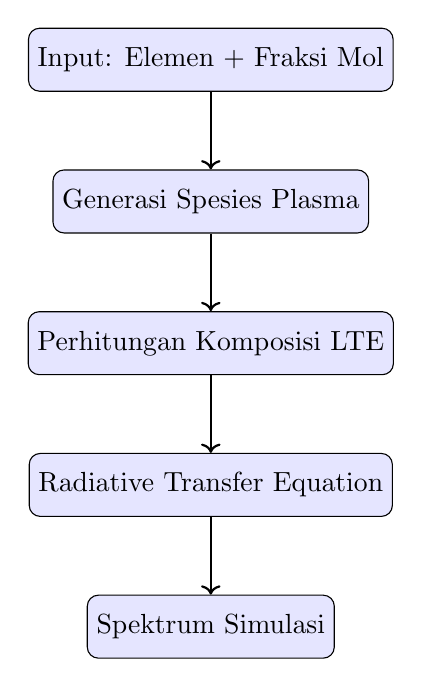
\begin{tikzpicture}[
      node distance=1.8cm,
      block/.style={draw, rounded corners, fill=blue!10, minimum width=3cm, minimum height=0.8cm},
      arrow/.style={->, thick}
    ]
      \node[block] (input) {Input: Elemen + Fraksi Mol};
      \node[block, below of=input] (species) {Generasi Spesies Plasma};
      \node[block, below of=species] (lte) {Perhitungan Komposisi LTE};
      \node[block, below of=lte] (rte) {Radiative Transfer Equation};
      \node[block, below of=rte] (spectra) {Spektrum Simulasi};

      \draw[arrow] (input) -- (species);
      \draw[arrow] (species) -- (lte);
      \draw[arrow] (lte) -- (rte);
      \draw[arrow] (rte) -- (spectra);
    \end{tikzpicture}
  \end{center}

  \vspace{6pt}

  \begin{block}{Ide Utama}
    MERLIN menggabungkan perhitungan komposisi plasma pada kondisi LTE
    dengan persamaan transfer radiasi untuk menghasilkan spektrum
    emisi plasma secara fisik konsisten.
  \end{block}
\end{frame}

% ──────────────────────────────────────────────────────────
\section{Landasan Teori}
% ──────────────────────────────────────────────────────────

\begin{frame}{2. Landasan Teori: Kerangka Umum MERLIN}
  \begin{center}
    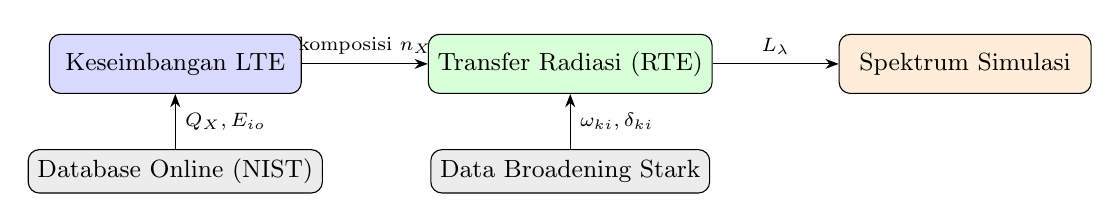
\begin{tikzpicture}[>=Stealth, font=\small, node distance=1.0cm]
      \node[draw, fill=blue!15, rounded corners, minimum width=3.2cm, minimum height=0.75cm]
            (lte) {Keseimbangan LTE};
      \node[draw, fill=green!15, rounded corners, minimum width=3.2cm, minimum height=0.75cm, right=1.6cm of lte]
            (rtc) {Transfer Radiasi (RTE)};
      \node[draw, fill=orange!15, rounded corners, minimum width=3.2cm, minimum height=0.75cm, right=1.6cm of rtc]
            (spec) {Spektrum Simulasi};
      \draw[->] (lte) -- node[above, font=\scriptsize]{komposisi $n_X$} (rtc);
      \draw[->] (rtc) -- node[above, font=\scriptsize]{$L_\lambda$} (spec);

      \node[draw, fill=gray!15, rounded corners, minimum width=3.2cm, minimum height=0.55cm, below=0.7cm of lte]
            (db) {Database Online (NIST)};
      \draw[->] (db) -- node[right, font=\scriptsize]{$Q_X, E_{io}$} (lte);

      \node[draw, fill=gray!15, rounded corners, minimum width=3.2cm, minimum height=0.55cm, below=0.7cm of rtc]
            (broad) {Data Broadening Stark};
      \draw[->] (broad) -- node[right, font=\scriptsize]{$\omega_{ki}, \delta_{ki}$} (rtc);
    \end{tikzpicture}
  \end{center}
  \vspace{4pt}
  \begin{columns}[T]
    \begin{column}{0.5\textwidth}
      \textbf{2.1 Komposisi Keseimbangan LTE}
      \begin{itemize}\small
        \item Sistem ODE kinetik fiktif (regex-based)
        \item Penurunan potensial ionisasi (Griem)
        \item Konstanta keseimbangan $K_{eq}$
      \end{itemize}
    \end{column}
    \begin{column}{0.5\textwidth}
      \textbf{2.2 Transfer Radiasi}
      \begin{itemize}\small
        \item Emisi bebas-terikat / bebas-bebas
        \item Emisi terikat-terikat (transisi diskret)
        \item Profil Voigt semu (pseudo-Voigt)
        \item Pelebaran Stark + pergeseran
      \end{itemize}
    \end{column}
  \end{columns}
\end{frame}

\begin{frame}{2.1 Kalkulasi Komposisi LTE}
  \begin{columns}[T]
    \begin{column}{0.55\textwidth}
      \begin{block}{Generasi Sistem ODE Adaptif}
        \begin{itemize}
          \item Reaksi fiktif: $R + M \underset{k_b}{\overset{k_f}{\rightleftharpoons}} P_1 + P_2 + M$
          \item Sistem ODE untuk setiap spesies $X$:
        \end{itemize}
        \vspace{2pt}
        \begin{equation}
          \frac{dN_R}{dt} = k_f\left(-N_R + K_{eq}^{-1}\,N_{P_1}\,n_{P_2}\,n_M\right) \tag{3a}
        \end{equation}
        \begin{itemize}
          \item Hingga \textbf{ratusan ODE} untuk campuran kompleks
          \item Ekuivalen dengan minimasi energi Gibbs
        \end{itemize}
      \end{block}
      \begin{exampleblock}{Konstanta Keseimbangan}
        \small
        \begin{equation}
          K_{eq} = \frac{Q_{P_1}Q_{P_2}}{Q_R}\left(\frac{2\pi\mu k_BT}{h^2}\right)^{3/2}
          \exp\!\left(\!-\frac{\delta_{r,io}E_{io}^c + \delta_{r,di}E_{di}}{k_BT}\right)
        \end{equation}
      \end{exampleblock}
    \end{column}
    \begin{column}{0.42\textwidth}
      \begin{alertblock}{Koreksi Penurunan Potensial Ionisasi}
        \small Pendekatan Griem untuk plasma lemah terionisasi:
        \begin{equation}
          \Delta E_{io}[\text{eV}] = \frac{Ze^2}{4\pi\epsilon_0}\sqrt{\frac{(Z+1)\,n_e}{\epsilon_0 k_B T}}
        \end{equation}
      \end{alertblock}
      \vspace{6pt}
      \begin{block}{Dua Mode Penyelesaian}
        \begin{enumerate}\small
          \item \textbf{Konstan $(T, p)$}: volume plasma berubah
          \item \textbf{Konstan $(T, n_X)$}: densitas tertentu tetap
        \end{enumerate}
      \end{block}
      \vspace{4pt}
      {\scriptsize Data fungsi partisi dan potensial ionisasi dari \textbf{NIST Atomic Spectra Database}}
    \end{column}
  \end{columns}
\end{frame}

\begin{frame}{2.2 Transfer Radiasi: Persamaan Dasar}
  \begin{block}{Persamaan Transfer Radiasi (RTE)}
    \begin{equation}
      \frac{dL_\lambda}{ds} = \epsilon_\lambda - \alpha_\lambda L_\lambda
    \end{equation}
    dengan $L_\lambda$ = radiansi spektral, $\epsilon_\lambda$ = koefisien emisi, $\alpha_\lambda$ = koefisien absorpsi
  \end{block}

  \vspace{4pt}
  \begin{columns}[T]
    \begin{column}{0.48\textwidth}
      \begin{block}{Geometri 2-Lapis MERLIN}
        \small
        Lapisan 1 (plasma panas): ketebalan $\ell_1$, $(T_1, n_{e,1})$\\
        Lapisan 2 (cold layer opsional): ketebalan $\ell_2$
        \begin{equation}
          L_{\lambda,T}^1 = \frac{\epsilon_{\lambda_1}}{\alpha_{\lambda_1}}\left(1-e^{-\alpha_{\lambda_1}\ell_1}\right)
        \end{equation}
        Kondisi \textbf{optically thin} ($\alpha_\lambda \ell_1 \ll 1$):
        \begin{equation}
          L_{\lambda,T}^1 \approx \epsilon_{\lambda_1}\ell_1
        \end{equation}
      \end{block}
    \end{column}
    \begin{column}{0.48\textwidth}
      \begin{block}{Komponen Koefisien Emisi}
        \small
        \begin{equation}
          \epsilon_{\lambda,X} = \underbrace{\epsilon_{\lambda,X}^{cont}}_{\text{kontinu}} + \underbrace{\sum_{ki}\epsilon_{\lambda,X}^{ki}}_{\text{diskret}}
        \end{equation}
        \begin{itemize}
          \item \textbf{Kontinu}: rekombinasi bebas-terikat ($fb$) + Bremsstrahlung ($ff$)
          \item \textbf{Diskret}: transisi spontan $k \to i$ (statistik Boltzmann)
        \end{itemize}
      \end{block}
    \end{column}
  \end{columns}
\end{frame}

\begin{frame}{2.2 Emisi Kontinu dan Diskret}
  \begin{columns}[T]
    \begin{column}{0.5\textwidth}
      \begin{block}{Emisi Bebas-Terikat (Rekombinasi Radiatif)}
        \footnotesize
        \begin{equation}
          \epsilon_{\lambda,X}^{fb(Z+)} = Z^2\frac{C_1 g_0^{X^{(Z+)}}}{Q_{X^{(Z+)}}\sqrt{T}\,\lambda^2}
          n_e n_{X^{(Z+)}}\!\left[1-e^{-\frac{hc}{\lambda k_BT}}\right]\xi^{fb}
        \end{equation}
      \end{block}
      \vspace{4pt}
      \begin{block}{Emisi Diskret (Transisi Terikat-Terikat)}
        \footnotesize
        Populasi level tereksitasi (Boltzmann):
        \begin{equation}
          [X_k] = \frac{g_k}{Q_X}\exp\!\left(-\frac{E_k}{k_BT}\right) n_X
        \end{equation}
        Koefisien emisi transisi $k\to i$:
        \begin{equation}
          \epsilon_{\lambda,X}^{ki} = \frac{hc\,A_{ki}[X_k]}{4\pi\,\lambda_{ki}}\,\Gamma(\lambda)
        \end{equation}
      \end{block}
    \end{column}
    \begin{column}{0.46\textwidth}
      \begin{exampleblock}{Profil Spektral: Pseudo-Voigt}
        \small
        Konvolusi Gaussian $\otimes$ Lorentzian $\Rightarrow$ \textbf{profil Voigt}\\
        Approksimasi polinomial (deviasi $<1\%$):
        \begin{itemize}\scriptsize
          \item Efisiensi: $\sim$\SI{10}{s} vs \SI{60}{min} (konvolusi langsung)
          \item Untuk tungsten, 4200 transisi, $[300, 800]$ nm
        \end{itemize}
      \end{exampleblock}
      \vspace{4pt}
      \begin{alertblock}{Sumber Pelebaran Garis}
        \scriptsize
        \begin{tabular}{ll}
          \toprule
          Sumber & Profil \\
          \midrule
          Aparatus ($\Delta\lambda_A$) & Lorentz \\
          Doppler ($\Delta\lambda_D$) & Gauss \\
          Van der Waals ($\Delta\lambda_{VdW}$) & Lorentz \\
          Resonansi ($\Delta\lambda_{Res}$) & Lorentz \\
          \redalert{Stark ($\Delta\lambda_{St}$)} & Lorentz \\
          \bottomrule
        \end{tabular}
      \end{alertblock}
    \end{column}
  \end{columns}
\end{frame}

\begin{frame}{2.2 Pelebaran Stark: Komponen Kunci CF-LIBS}
  \begin{columns}[T]
    \begin{column}{0.52\textwidth}
      \begin{block}{FWHM Stark (Teori Griem)}
        \footnotesize
        \begin{equation}
          \Delta\lambda_{ki}^{St} = 2\omega_{ki}(T)\frac{n_e}{n_{e,r}}
          \left[1 + 1.75\,A_S(T)\!\left(\frac{n_e}{n_{e,r}}\right)^{1/4}\!\!\left(1-\frac{3}{4}N_D^{-1/3}\right)\right]
        \end{equation}
        dengan $\omega_{ki}(T)$ = faktor impact Stark\\
        $n_{e,r} = 10^{22}$ m$^{-3}$ = densitas referensi
      \end{block}
      \begin{block}{Pergeseran Stark ($\delta\lambda_{ki}$)}
        \footnotesize
        \begin{equation}
          \delta\lambda_{ki} = \omega_{ki}(T)\left[1.4 + 2A_S(T)\left(\frac{n_e}{n_{e,r}}\right)^{1/4}\!\!\left(1-N_D^{-1/3}\right)\right]
        \end{equation}
      \end{block}
    \end{column}
    \begin{column}{0.44\textwidth}
      \begin{exampleblock}{Pentingnya Stark dalam LIP}
        \begin{itemize}\small
          \item Stark \textbf{dominan} untuk $n_e \gtrsim 5\times10^{22}$ m$^{-3}$
          \item Digunakan untuk mengukur $n_e$ secara eksperimental
          \item Transisi Ar~II dan H~I 656.28 nm digunakan
        \end{itemize}
      \end{exampleblock}
      \vspace{4pt}
      \begin{alertblock}{Koreksi Self-Absorpsi}
        \footnotesize
        Faktor koreksi:
        \begin{equation}
          C_{ki}^{SA} = \frac{\int(1-e^{-\alpha_\lambda \ell_1})d\lambda}{\int \alpha_\lambda \ell_1\, d\lambda}
        \end{equation}
        Prosedur iteratif untuk konvergensi $n_e$
      \end{alertblock}
    \end{column}
  \end{columns}
\end{frame}

% ──────────────────────────────────────────────────────────
\section{Validasi Eksperimental}
% ──────────────────────────────────────────────────────────

\begin{frame}{3. Validasi: Platform Eksperimental PLEIADES}
  \begin{columns}[T]
    \begin{column}{0.55\textwidth}
      \begin{block}{Setup Eksperimental (Laboratorium CORIA)}
        \begin{itemize}\small
          \item Laser: QUANTEL Briant B Nd:YAG
          \item Target: Eurofer97 (baja reduksi aktivasi)
          \item Atmosfer: Ar, $p = \SI{5e4}{Pa}$
          \item Akuisisi: sinkron per tembakan, 10 tembakan/spektrum
        \end{itemize}
      \end{block}
      \vspace{4pt}
      \begin{exampleblock}{Parameter Laser}
        \small
        \begin{tabular}{ll}
          \toprule
          Parameter & Nilai \\
          \midrule
          Panjang gelombang & \SI{1064}{nm} \\
          Energi & \SI{45}{mJ} \\
          Durasi pulsa & \SI{6.0}{ns} \\
          Laju repetisi & \SI{10}{Hz} \\
          Fluensi puncak & $\SI{160\pm50}{J.cm^{-2}}$ \\
          Fluks puncak & $\SI{2.5e14}{W.m^{-2}}$ \\
          \bottomrule
        \end{tabular}
      \end{exampleblock}
    \end{column}
    \begin{column}{0.42\textwidth}
      \begin{block}{Sistem Deteksi}
        \small
        \begin{tabular}{ll}
          \toprule
          Komponen & Spesifikasi \\
          \midrule
          Spektrometer & SCT-320, $f=\SI{320}{mm}$ \\
          Kisi & 600 \& 3600 g/mm \\
          Kamera VUV & PI-MAX 4, 13\% QE @ 274nm \\
          Kamera Vis & PI-MAX 4, 37\% QE @ 650nm \\
          Fiber optik & 19 serat, \O{}200 $\mu$m \\
          Resolusi waktu & \SI{50}{ns}/jendela \\
          \bottomrule
        \end{tabular}
      \end{block}
      \vspace{4pt}
      {\scriptsize Kalibrasi radiometrik: lampu H$_2$D$_2$ ($\lambda<\SI{400}{nm}$) dan lampu pita W ($\lambda>\SI{400}{nm}$)}
    \end{column}
  \end{columns}
\end{frame}

\begin{frame}{3. Komposisi Sampel Eurofer97}
  \begin{columns}[T]
    \begin{column}{0.48\textwidth}
      \begin{block}{Fraksi Mol Eurofer97}
        \small
        \begin{tabular}{lcc}
          \toprule
          Elemen & $x_{X,XRF}$ (ref.) & $x^*_{X,LIBS}$ \\
          \midrule
          Fe & 0.8530 & (major) \\
          Cr & 0.0977 & \\
          Cu & 0.0222 & \\
          W  & --- & \\
          Mn & --- & \\
          V  & --- & \\
          \bottomrule
          \multicolumn{3}{l}{\scriptsize Elemen $<500$ ppm tidak dimasukkan}
        \end{tabular}
      \end{block}
    \end{column}
    \begin{column}{0.48\textwidth}
      \begin{alertblock}{Tantangan Sampel}
        \begin{itemize}\small
          \item Baja kompleks dengan 11 elemen terukur (XRF)
          \item Elemen minor: Cu, W, Na, Mn, V, Se, Co, K, Zn
          \item Perlu dekonvolusi garis spektral yang tumpang tindih
        \end{itemize}
      \end{alertblock}
      \vspace{6pt}
      \begin{exampleblock}{Strategi Rekonstruksi MERLIN}
        \begin{itemize}\small
          \item Tanpa variabel penyesuaian
          \item Input: $T$, $n_e$, komposisi dari pengukuran
          \item Output: spektrum simulasi vs eksperimental
        \end{itemize}
      \end{exampleblock}
    \end{column}
  \end{columns}
\end{frame}

\begin{frame}{3.2--3.3 Benchmark LTE dan Dinamika Plasma}
  \begin{columns}[T]
    \begin{column}{0.5\textwidth}
      \begin{block}{Benchmark Komposisi LTE}
        \small
        \textbf{Campuran udara}: $0.2115$ O$_2 + 0.7885$ N$_2$\\
        $p = \SI{e5}{Pa}$, $T$ bervariasi\\[4pt]
        Hasil MERLIN vs literatur:
        \begin{itemize}
          \item Sangat baik untuk spesies netral dan bermuatan
          \item Deviasi kecil untuk NO, NO$_2$ saat $T < \SI{3000}{K}$\\
                (akibat perbedaan database termokimia)
        \end{itemize}
      \end{block}
    \end{column}
    \begin{column}{0.5\textwidth}
      \begin{block}{Dinamika Geometri Plasma}
        \small
        Ketebalan plasma $\ell_1$ terhadap waktu (hukum pangkat):
        \begin{equation}
          \ell_1(t) = \ell_{1,0}\left(\frac{t}{t_0}\right)^B, \quad B = 0.191
        \end{equation}
        \begin{itemize}
          \item $\ell_{1,0} = \SI{645}{\micro m}$ pada $t_0 = \SI{10}{ns}$
          \item Kecepatan ekspansi awal: $\sim \SI{2e3}{m/s}$
          \item Kecepatan ekspansi akhir: $\sim \SI{3e2}{m/s}$
        \end{itemize}
      \end{block}
    \end{column}
  \end{columns}
  \vspace{6pt}
  \begin{alertblock}{Kriteria McWhirter (Verifikasi LTE)}
    \small
    Untuk Ar ($10^4 < T < 1.5\times10^4$ K): $n_e^{min} \in [2.46, 3.02]\times10^{23}$ m$^{-3}$\\
    Untuk Fe (struktur elektronik sangat padat): ambang $\sim$100$\times$ lebih rendah\\
    $\Rightarrow$ \textbf{LTE terpenuhi secara sistematis} dalam kondisi eksperimental kami
  \end{alertblock}
\end{frame}

\begin{frame}{3.4 Pengukuran Densitas Elektron $n_e$}
  \begin{columns}[T]
    \begin{column}{0.55\textwidth}
      \begin{block}{Metode: Pelebaran \& Pergeseran Stark}
        \small
        Transisi yang digunakan (Ar~II, Ar~I, H~I):
        \begin{tabular}{llll}
          \toprule
          Spesies & $\lambda$ (nm) & $\omega_{ki}$ (pm) & $\delta_{ki}$ (pm) \\
          \midrule
          Ar~II & 648.31 & 6.52 & 1.67 \\
          H~I   & 656.28 & 106.56 & 5.14 \\
          Ar~II & 664.37 & 7.18 & --- \\
          Ar~II & 668.43 & 6.16 & --- \\
          Ar~I  & 696.54 & 6.67 & 3.03 \\
          Ar~I  & 706.72 & 6.60 & 2.73 \\
          \bottomrule
        \end{tabular}
      \end{block}
    \end{column}
    \begin{column}{0.42\textwidth}
      \begin{block}{Hasil Interpolasi}
        \begin{equation}
          n_e(t) = n_{e,0}\left(\frac{t}{t_0}\right)^B
        \end{equation}
        \begin{itemize}\small
          \item $B = -1.105$
          \item $t_0 = \SI{10}{ns}$
          \item $n_{e,0} = 2.33\times10^{25}$ m$^{-3}$
        \end{itemize}
      \end{block}
      \begin{exampleblock}{Koreksi Self-Absorpsi}
        \small
        Iterasi $C_{ki}^{SA}$ (koefisien El Sherbini): $a=-0.54$, $b=0.46$\\
        Rata-rata tertimbang dari semua transisi
      \end{exampleblock}
    \end{column}
  \end{columns}
\end{frame}

\begin{frame}{3.5 Pengukuran Temperatur: Plot Saha-Boltzmann}
  \begin{columns}[T]
    \begin{column}{0.55\textwidth}
      \begin{block}{Metode Plot Saha-Boltzmann (SB)}
        \small
        Ordinat plot SB dari pengukuran radiansi garis:
        \[\text{Ordinat} \propto \ln\!\left(\frac{L_{ki}\lambda_{ki}}{g_k A_{ki}}\right) - \text{(koreksi $n_e$)}\]
        Kemiringan linear $\Rightarrow$ \textbf{suhu plasma $T$}\\[4pt]
        \begin{itemize}
          \item Transisi Fe~I, Fe~II, Ar~I, Ar~II digunakan
          \item Linearitas plot memverifikasi LTE
          \item Koreksi self-absorpsi diterapkan
        \end{itemize}
      \end{block}
    \end{column}
    \begin{column}{0.42\textwidth}
      \begin{block}{Rentang Kondisi Terukur}
        \begin{center}
          \begin{tabular}{lll}
            \toprule
            Waktu & $T$ (K) & $n_e$ (m$^{-3}$) \\
            \midrule
            Awal & $\sim\!1.5\times10^4$ & $\sim\!10^{25}$ \\
            Tengah & $\sim\!1.2\times10^4$ & $\sim\!10^{24}$ \\
            Akhir & $\sim\!8\times10^3$ & $\sim\!10^{22}$ \\
            \bottomrule
          \end{tabular}
        \end{center}
      \end{block}
      \begin{alertblock}{Pemilihan Transisi Optis Tipis}
        \small
        Hanya transisi dengan $C_{ki}^{SA} \approx 1$ yang dipertahankan untuk mengukur $T$ secara akurat
      \end{alertblock}
    \end{column}
  \end{columns}
\end{frame}

% ──────────────────────────────────────────────────────────
\section{Rekonstruksi Spektrum \& Hasil}
% ──────────────────────────────────────────────────────────

\begin{frame}{3.6 Rekonstruksi Spektrum dengan MERLIN}
  \begin{block}{Prosedur Rekonstruksi (Tanpa Variabel Bebas)}
    \begin{enumerate}\small
      \item Ukur $n_e(t)$ dari pelebaran Stark Ar~II dan H~I
      \item Ukur $T(t)$ dari plot Saha-Boltzmann
      \item Ukur $\ell_1(t)$ dari citra spasial plasma
      \item Input $(T, n_e, \ell_1, x_X)$ ke MERLIN $\Rightarrow$ hitung $L_\lambda^{sim}$
      \item Bandingkan langsung $L_\lambda^{sim}$ vs $L_\lambda^{exp}$
    \end{enumerate}
  \end{block}

  \vspace{4pt}
  \begin{columns}[T]
    \begin{column}{0.48\textwidth}
      \begin{exampleblock}{Rentang Spektral Dianalisis}
        \begin{itemize}\small
          \item Grating 3600 g/mm: $[260\text{--}290]$ nm (UV)
          \item Grating 600 g/mm: $[600\text{--}750]$ nm (VIS-NIR)
          \item Fokus pada garis Fe, Cr, W, Ar
        \end{itemize}
      \end{exampleblock}
    \end{column}
    \begin{column}{0.48\textwidth}
      \begin{alertblock}{Kriteria Keberhasilan}
        \begin{itemize}\small
          \item Tidak ada penyesuaian \textit{post-hoc}
          \item Setiap garis spektral harus cocok secara amplitudo dan lebar
          \item Validasi di berbagai waktu tunda (temporal)
        \end{itemize}
      \end{alertblock}
    \end{column}
  \end{columns}

  \vspace{6pt}
  {\small \textbf{Hasil}: MERLIN berhasil merekonstruksi spektrum emisi plasma Eurofer97 dalam Ar pada berbagai waktu tanpa variabel penyesuaian. Persetujuan baik antara spektrum simulasi dan eksperimental.}
\end{frame}

\begin{frame}{Pengaruh Database Spektral}
  \begin{columns}[T]
    \begin{column}{0.55\textwidth}
      \begin{block}{Database yang Digunakan MERLIN}
        \small
        \begin{tabular}{ll}
          \toprule
          Database & Data \\
          \midrule
          \textbf{NIST ASD} & $Q_X(T)$, $E_{io}$, $A_{ki}$, $E_k$, $g_k$ \\
          \textbf{DESIRE} & Transisi W, Cr (metal berat) \\
          Wilbers et al. & Faktor Bibermann $\xi^{fb}$ \\
          Devoto & $\sigma_{ea}(T)$ (penampang elastik $e$-atom) \\
          \bottomrule
        \end{tabular}
      \end{block}
      \vspace{4pt}
      \begin{block}{Nilai yang Digunakan}
        \small
        \begin{itemize}
          \item $\xi^{fb}(\lambda,T,Z) = 1.75$ (argon, rata-rata)
          \item $\sigma_{ea}(T) = 3\times10^{-19}$ m$^2$
          \item $\xi^{ff}(\lambda,T,Z) = 1$ (grafik Sutherland)
        \end{itemize}
      \end{block}
    \end{column}
    \begin{column}{0.42\textwidth}
      \begin{alertblock}{Keterbatasan Database}
        \begin{itemize}\small
          \item Nilai $\xi^{fb}$ dan $\sigma_{ea}$ tersedia hanya untuk Ar
          \item Asumsi nilai rata-rata untuk spesies lain
          \item Untuk transisi optis tipis yang dominan: pengaruh linear terhadap $L_\lambda$
        \end{itemize}
      \end{alertblock}
      \vspace{6pt}
      \begin{exampleblock}{Kemampuan Multi-Database}
        \small
        MERLIN dapat kueri \textbf{beberapa database secara otomatis} dan melakukan kalkulasi multi-basis, meningkatkan kelengkapan data atomik
      \end{exampleblock}
    \end{column}
  \end{columns}
\end{frame}

\begin{frame}{Hasil Utama Penelitian}
  \begin{block}{Validasi Model}
    \begin{itemize}
      \item Komposisi LTE berhasil divalidasi menggunakan benchmark
            campuran udara.
      \item Parameter plasma seperti temperatur dan densitas elektron
            diperoleh dari pengukuran eksperimen.
      \item Spektrum simulasi menunjukkan kesesuaian yang baik dengan
            spektrum eksperimen LIBS.
    \end{itemize}
  \end{block}

  \begin{exampleblock}{Kinerja Model}
    \begin{itemize}
      \item Rekonstruksi spektrum pada rentang UV dan VIS
      \item Korelasi simulasi--eksperimen mencapai
            \textbf{> 99\%} pada beberapa rentang spektral
    \end{itemize}
  \end{exampleblock}
\end{frame}

% ──────────────────────────────────────────────────────────
\section{Diskusi \& Kesimpulan}
% ──────────────────────────────────────────────────────────

\begin{frame}{Keterbatasan Pendekatan}
  \begin{alertblock}{Batasan Model}
    \begin{itemize}
      \item Model mengasumsikan kondisi
            \textbf{Local Thermodynamic Equilibrium (LTE)}
      \item Beberapa parameter kontinu menggunakan nilai pendekatan
      \item Data pelebaran Stark tidak selalu tersedia untuk semua garis
      \item Model dua lapis plasma masih memerlukan parameter tambahan
    \end{itemize}
  \end{alertblock}

  \begin{block}{Implikasi}
    Keterbatasan ini menunjukkan peluang pengembangan lebih lanjut,
    misalnya integrasi model \textit{non-LTE} atau peningkatan basis
    data atomik untuk simulasi spektrum.
  \end{block}
\end{frame}

\begin{frame}{Diskusi: Kelebihan dan Keterbatasan MERLIN}
  \begin{columns}[T]
    \begin{column}{0.5\textwidth}
      \begin{exampleblock}{\textcolor{green!50!black}{$\checkmark$} Kelebihan MERLIN}
        \begin{enumerate}\small
          \item \textbf{Adaptif}: campuran elemen apapun, jumlah spesies tidak dibatasi
          \item \textbf{Otonom}: query database online secara otomatis
          \item \textbf{Efisien}: pseudo-Voigt (1600$\times$ lebih cepat dari konvolusi langsung)
          \item \textbf{Paralel}: berjalan di mesin kapasitas rendah
          \item \textbf{Rigorous}: tidak ada variabel bebas dalam rekonstruksi
          \item \textbf{Poliatom}: spesies poliatom didukung (tidak dipresentasikan)
        \end{enumerate}
      \end{exampleblock}
    \end{column}
    \begin{column}{0.5\textwidth}
      \begin{alertblock}{\textcolor{red!70!black}{$\triangle$} Keterbatasan \& Asumsi}
        \begin{enumerate}\small
          \item LTE diasumsikan (terverifikasi via McWhirter)
          \item Nilai $\xi^{fb}$ dan $\sigma_{ea}$ diasumsikan dari Ar (ideal hidrogen)
          \item Koreksi Virial/Debye-Hückel terhadap persamaan keadaan tidak dimasukkan
          \item Fungsi partisi dihitung tanpa ketergantungan densitas
          \item Ketidakpastian data Stark dari literatur propagasi ke $n_e$
        \end{enumerate}
      \end{alertblock}
    \end{column}
  \end{columns}
\end{frame}

\begin{frame}{Kesimpulan}
  \begin{block}{Ringkasan Kontribusi Utama}
    \begin{enumerate}
      \item \textbf{Pengembangan MERLIN}: kode transfer radiasi LTE adaptif untuk campuran elemen apapun, lengkap dengan penanganan emisi kontinu (fb/ff) dan diskret, pelebaran dan pergeseran Stark
      \item \textbf{Validasi komprehensif} pada Eurofer97 dalam atmosfer Ar:
            \begin{itemize}
              \item Komposisi LTE vs referensi literatur (campuran udara): $\checkmark$
              \item Dinamika $n_e(t)$ via Stark: $\checkmark$
              \item Temperatur $T(t)$ via Saha-Boltzmann: $\checkmark$
              \item Rekonstruksi spektrum simulasi vs eksperimen: $\checkmark$
            \end{itemize}
      \item \textbf{Tanpa variabel penyesuaian}: semua input dari pengukuran independen
    \end{enumerate}
  \end{block}
  \vspace{4pt}
  \begin{exampleblock}{Implikasi untuk CF-LIBS}
    MERLIN siap digunakan untuk \textbf{karakterisasi komposisi sampel kompleks} melalui CF-LIBS, dengan basis fisika yang solid dan kemampuan generalisasi tinggi.
  \end{exampleblock}
  \begin{flushright}
    \small \textit{Journal of Quantitative Spectroscopy \& Radiative Transfer} \textbf{330} (2025) 109222\\
    A. Favre, B. Brioude, A. Bultel --- CORIA UMR 6614, Rouen
  \end{flushright}
\end{frame}

\begin{frame}{Referensi Kunci}
  \begin{columns}[T]
    \begin{column}{0.5\textwidth}
      \textbf{Teori \& Fisika Plasma}
      \begin{enumerate}\scriptsize
        \item Stewart \& Pyatt --- ionization potential lowering
        \item Griem --- Stark broadening theory
        \item Prenzel et al. --- ideal gas EOS validity ($T < 10^5$ K)
        \item El Sherbini et al. --- self-absorption correction
        \item McWhirter --- LTE criterion
      \end{enumerate}
      \vspace{6pt}
      \textbf{Database Atomik}
      \begin{enumerate}\scriptsize
        \setcounter{enumi}{5}
        \item NIST Atomic Spectra Database \url{physics.nist.gov}
        \item DESIRE --- database for W and Cr transitions
        \item Wilbers et al. --- Bibermann factors for Ar
        \item Devoto --- electron-neutral cross-sections
      \end{enumerate}
    \end{column}
    \begin{column}{0.5\textwidth}
      \textbf{Validasi \& Benchmark}
      \begin{enumerate}\scriptsize
        \setcounter{enumi}{9}
        \item Artikel utama: Favre et al., JQSRT 330 (2025) 109222
        \item Platform PLEIADES, CORIA laboratory, Rouen
        \item Eurofer97 reference: XRF composition data [Table 2]
      \end{enumerate}
      \vspace{8pt}
      \begin{alertblock}{Kata Kunci untuk Pencarian}
        \scriptsize
        CF-LIBS $\cdot$ Radiative Transfer $\cdot$ LTE $\cdot$\\
        Stark Broadening $\cdot$ Plasma Diagnostics $\cdot$\\
        Eurofer97 $\cdot$ MERLIN code $\cdot$ Spectral simulation
      \end{alertblock}
    \end{column}
  \end{columns}
\end{frame}

% ── Penutup ───────────────────────────────────────────────
\begin{frame}[plain]
  \begin{center}
    \vspace{1.5cm}
    {\Huge \textbf{Terima Kasih}}\\[1cm]
    {\large \textit{Pertanyaan dan Diskusi}}\\[1.5cm]
    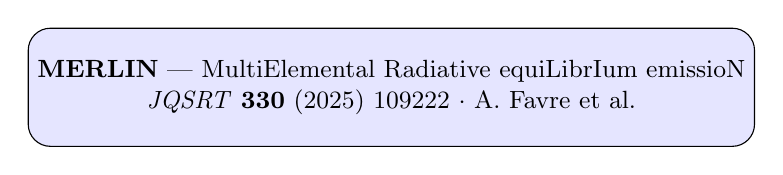
\begin{tikzpicture}
      \node[draw, fill=blue!10, rounded corners=8pt, minimum width=8cm, minimum height=1.5cm,
            align=center, font=\small]{%
        \textbf{MERLIN} --- MultiElemental Radiative equiLibrIum emissioN\\
        \textit{JQSRT} \textbf{330} (2025) 109222 $\cdot$ A. Favre et al.};
    \end{tikzpicture}
  \end{center}
\end{frame}

\end{document}
